\documentclass[tikz,border=8pt]{standalone}
\usepackage{amsmath,amssymb}
\usetikzlibrary{arrows.meta,automata,positioning,quotes}
\begin{document}
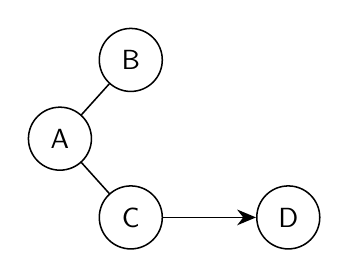
\begin{tikzpicture}[x=1cm,y=1cm]
\tikzset{
  graphnode/.style={circle,draw=black,line width=0.55pt,minimum size=8mm,inner sep=1pt,font=\sffamily},
  graphedge/.style={draw=black,line width=0.55pt,line cap=round,line join=round},
  directed/.style={graphedge,-{Stealth[length=2.4mm,width=2.0mm]}},
  undirected/.style={graphedge}
}
\node[graphnode] (n_A) at (1.10,0.00) {A};
\node[graphnode] (n_B) at (2.00,1.00) {B};
\node[graphnode] (n_C) at (2.00,-1.00) {C};
\node[graphnode] (n_D) at (4.00,-1.00) {D};
\draw[undirected] (n_A) -- (n_B);
\draw[undirected] (n_A) -- (n_C);
\draw[directed] (n_C) -- (n_D);
\end{tikzpicture}
\end{document}
